\documentclass[a4paper,12pt]{article}
\usepackage[latin1]{inputenc}
%\usepackage[spanish]{babel}
\usepackage{amssymb}
\usepackage{graphicx}
%\usepackage{textcomp}
\usepackage{geometry}
\geometry{margin=1in}
\usepackage{cite}
\usepackage{url}
\usepackage{hyperref}
\usepackage{float}
\usepackage{amsmath}
\usepackage{cleveref}

\crefformat{footnote}{#2\footnotemark[#1]#3}

\title{\textbf{Currency exchange rates analysis}}
\author{Miguel Tasende}

%opening
\begin{document}


\maketitle

\section{Abstract}
Uruguay has a semi-dollarized economy: salaries and basic goods are normally traded in UYU but the larger ones (houses, cars, home appliances, etc) are traded in USD. Historically, middle-income Uruguayans have had very few investment instruments available, or at very high costs, so, a typical middle-income family or individual would normally save in USD, or in ``Indexed UYU'' (UI) if expecting to buy a house, for example. In that scenario a typical question is ``which one is better? USD or UI?''. In this work the convenience of saving in USD or UI was studied making use of the PPP theory, Bayesian statistics, hierarchical models, and some simplifications. It was confirmed that the UYU is more likely to be overvalued in its present value\footnote{The last value in the dataset: December, 2016\label{ref1}} than not (with the limited data and models used), a 95\% confidence interval was calculated for the mean of the UYU/USD exchange rate, as well as for the rate itself. Finally, it was determined whether it is more convenient to save in USD or UI, depending on the current exchange rate and value of the US inflation in one year.

\section{Introduction}
The chosen problem will be addressed from a local perspective, even if the same procedures can be generalized to any other countries in the dataset. The questions to answer are: 
\begin{itemize}
\item Is Uruguay's currency overvalued or undervalued with respect to the U.S. Dollar? Which is the probability that the UYU is overvalued/undervalued?
\item In which equally tailed interval is the UYU/USD rate supposed to be in, for the last date available in the dataset (December, 2016), with a 95\% probability?
\item For a Uruguayan (someone who earns the salary in UYU), is it more convenient to save in USD or in ``Inflation Indexed UYU'' (UI) for one year? If so, which is the probability that saving in USD is more convenient than saving in UI?
\end{itemize}
In this work some (rather big) simplifications will be made:
\begin{enumerate}
\item The Parity Purchase Power theory will be used as a theoretical background, in its simplest version.
\item The time dependence of the exchange rate deviations will be completely ignored (i.e.: deviations from the PPP theory are assumed to be stationary).
\item Exchange fees are ignored.
\end{enumerate}

\section{Data}
It was decided to try to collect the exchange rate ($\frac{Currency}{USD}$) for every country and every date that was possible. Also the CPI (Consumer Price Index) for every country and date available, was searched for, to make use of the PPP theory. Finally the country's name and region for each currency was also searched for, as a region-based model was consiered. The sources were:
\begin{itemize}
\item Exchange rates: Pacific Exchange Rate service \\(\verb+(C) 2017 Prof. Werner Antweiler, UBC+)
\item CPI: International Monetary Fund
\item Regions: World Bank
\end{itemize}
As there were three sources for the data, it was necessary to standarize it. In particular the dates were standarized, and the (unique) currency codes used as indexes. In some cases it was necessary to fill the codes manually. Then missing data was studied, for the exchange rates first. It was decided to use only the period from 2007 to 2017, as it contained many currencies without missing data. The currencies that had exchange rate missing data in that period were dropped. Another problem was that some currencies were used in more than one country. In those cases, the country with a clearly larger population and GDP was chosen as the currency's country. In one case it was not possible to decide wich country was the representative one and the currency was dropped. After that, some countries that had adopted dollar parity were dropped. Then the resulting list was joined with the CPI list. Those countries that had missing CPI data were also dropped. Also, some countries seemed to report the CPI quarterly instead of monthly (Australia, New Zealand, Kingdom of Bahrain) and were dropped too. 
\\The data is for 51 countries between the years 2007 and 2017, and it contains Exchange Rate, CPI, as well as country name, region, date, and currency code.

\begin{figure}[!h]
\centering
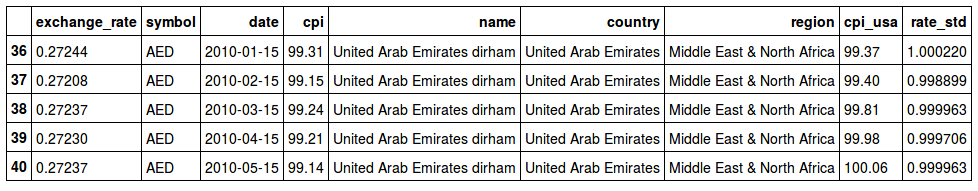
\includegraphics[width=4.5in]{images/i002_prep_data.png}
\caption{The first elements of the Preprocessed Data. rate\_std is the exchange rate divided by its value on August, 2010, for each currency.}
\label{fig_raw_data}
\end{figure}

To explore the data, some graphs were produced. The quotient $y = \frac{rate_{std} \times cpi}{cpi_{usa}}$ was studied: it's density and trace were plotted (after shuffling the data), a boxplot with the currency symbol as independent variable was produced, and the rate\_std vs cpi\_quotient graph. It could be seen that there is some noticeable variability between currencies, that there is a clear positive correlation between the CPI quotient and the standarized rates, and the density of the full quotient ($y$) seems to be multi-modal (a mixture model was not explored because the multimodality is easily explained with the different behaviours for different countries/regions).

\begin{figure}[!h]
\centering
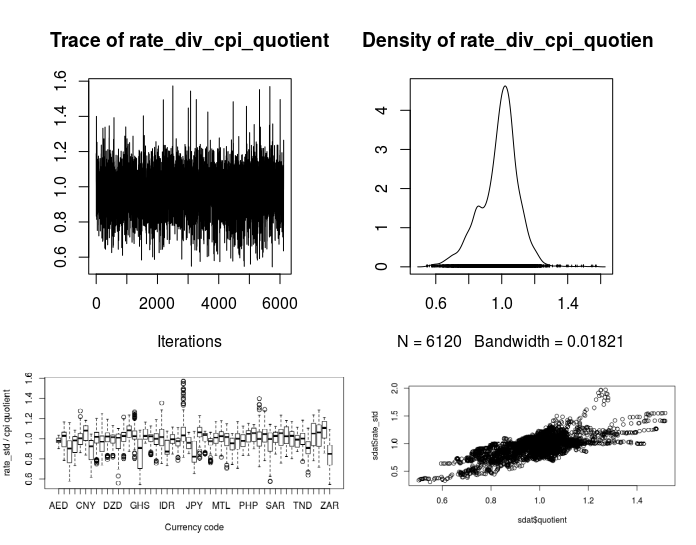
\includegraphics[width=3.5in]{images/i006_graphs_exploring.png}
\caption{Graphs showing the exploratory analysis}
\label{fig_raw_data}
\end{figure}


\section{Model}
A reference (linear) model and six JAGS models were studied. I will only give details for the one selected, but a resumed table with the DIC for all the models can be seen below (their name is descriptive):


\begin{tabular}{|p{2cm}|p{2cm}|p{2cm}|p{2cm}|p{2cm}|p{2cm}|p{2cm}|}
\hline
\textbf{Model} &1. ANOVA ($\mu$)&2. Hierarchical country ($\mu$)&3. ANOVA ($\mu$, $\sigma$)&4. Hierarchical country ($\mu$, $\sigma$)&5. Hierarchical region ($\mu$, $\sigma$)&6. Hierarchical region and country ($\mu$, $\sigma$) \\
\hline
\textbf{DIC} & -10374 & -9533 & -5647 & -11380 & -9671 & -11382 \\
\hline
\end{tabular}


Model 4 was chosen (Hierarchical country ($\mu$, $\sigma$)) because it has the same (lowest) DIC as model 6, but the convergence tests have better results for it and it is simpler.\\
Model 4 is a hierarchical model. The data ($y = \frac{rate_{std} \times cpi}{cpi_{usa}}$) is assumed normally distributed with one mean ($\mu_j$) and one standard deviation $\sigma_j$ for each country. The $\mu_j$'s are assumed to be normally distributed with mean and standard deviation $\mu_{\mu}$ and $\sigma_{\mu}$. The $\sigma_j^2$'s are assumed to follow an Inverse Gamma distribution with parameters $a_{\sigma}$ and $b_{\sigma}$. The chosen priors were:
$$
\mu_{\mu} \sim N(0, 10^{-6}) , \quad
\sigma_{\mu}^2 \sim IG(1/2, 10/2) , \quad
a_{\sigma} \sim Exp(100) , \quad
b_{\sigma} \sim Exp(100)
$$

\begin{figure}[!h]
\centering
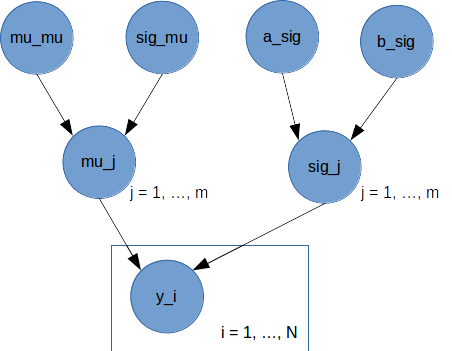
\includegraphics[width=2.0in]{images/i007_hierarchical.png}
\caption{Model representation.}
\label{fig_raw_data}
\end{figure}
The model is based on the PPP theory. It was asssumed that some parameters may have shared information between countries, even when they are different. The DIC seems to show that it is the case for both $\mu$ and $\sigma$. The priors were selected to be uninformative, conjugates if possible, positive in the case of $a_{\sigma}$ and $b_{\sigma}$.\\
The MCMC convergenge was assessed by using traceplots, autocorrelation diagnostics, effective size, Raftery diagnostics, Gelman and Rubin diagnostics. The results were very good for almost all parameters. As some of the parameters at the top of the hierarchy ($a_{\sigma}$) seemed to have some correlation for 5 to 10 lags, it was decided to use $7000$ samples for each chain (3 chains were used). The residuals analysis results showed no obvious correlation to index or values, and no outliers.

\section{Results \& Conclusions}

The expected value of the UYU/USD exchange rate, with the current \cref{ref1} CPI quotient is: 30.49 . The current\cref{ref1} value is: 28.7828, so the conclusion is that UYU is overvalued (the rate should be higher). The probability that it is overvalued is: 0.66 ($y$ values were simulated from the parameters to calculate that).\\
From the summary, after some calculations, the mean of the UYU/USD rate is in this equally tailed interval with probability 95\%: $[29.67277, 31.21428]$, on the other hand, the equally tailed interval with probability 95\% for the actual UYU/USD rate is: $[23.82859, 42.30231]$ (obs.: the current value is within the interval). Finally, the convenience of saving in USD or in Indexed UYU was assessed. The value of the USD inflation for which $P(y_1 < \frac{pciUSA_0}{pciUSA_1}y_0)$, where the ``1'' subindex corresponds to the value after one year, was calculated (the ``0'' index corresponds to the value in December, 2016). The result was that it would be convenient to buy USD instead of UI (in Dec, 2016), to hold them for a year, if and only if the inflation in the USA is less than 2.37\% . A complete graph for the probability that it is convenient to save in USD instead of UI, given the inflation in the USA, was also produced.

\begin{figure}[!h]
\centering
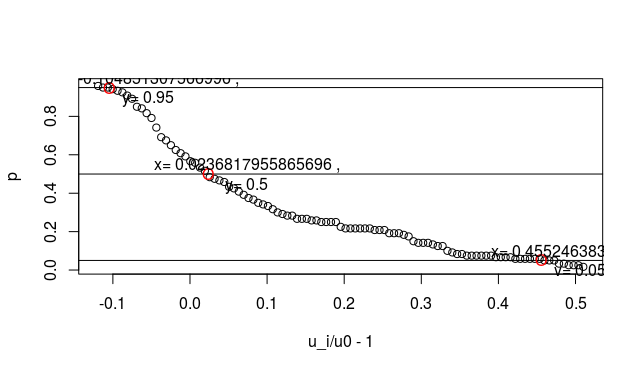
\includegraphics[width=3.5in]{images/i008_inflation.png}
\caption{Probability that USD is convenient over UI, for one year, as a function of inflation in the USA ($\frac{CPI_{USA}1}{CPI_{USA}0} - 1$).}
\label{fig_raw_data}
\end{figure}

\end{document}